

\section{Continuation}
\label{sec:continuation}

When the periodic solution is found, finding the successively periodic solutions
is done by continuation.

As with finding periodic solutions, there exist multiple schemes to do
continuation. A general continuation is formulated as $F(x)=0, \quad
F:\mathbb{R}^{m+1} \to \mathbb{R}^{m} $, ie. here the structure is $\bm z \in
\mathbb{R}^m$, $\omega \in \mathbb{R}^1$ and $F$ the algebraic problem for which
a solution is sought.

The most simple continuation method, where $\omega$ is used as independent
parameter and uniformly increased at each step fails at turning points. Instead
most continuation methods uses a length-wise curve parameter and a
predictor-corrector model. Starting from a known solution $\bm y_j = [\bm
z_{p0,(j)},\omega_{(j)}]^T$ the next periodic solution $\bm y_{j+1}$ is found as

\begin{itemize}
\item Tangent prediction, $\bm y_{(j+1)}^{1} = y_{(j)}+s\bm t_{(i)}$, where $s$
  is the step size and $\bm t$ the tangent.
\item Newton-like corrections - The type determines the continuation method.
\item Adaptive step control. Here a simple model using the convergence of the
  Newton iterations is used: $s = \frac{it_{opt}}{it_{NR}} s$, ie. the step is
  updated based on the defined optimal number of iterations versus the actual
  used number of iteration
\end{itemize}

The two methods used in this project are the pseudo-archlength continuation and
the Moore-Penrose continuation. The main difference is computional complexity.
With pseudo-archlength, each time a new point is found on the curve, the tangent
vector have to be computed anew. With the Moore-penrose corrector, the tangent
vector is also corrected and we save the explicit calculation of the tangent at
each new point.

The aim is to show that is no harder to use the Moore-penrose corrector. Formal
descriptions are found in \citet{dhooge2003a}

\subsection{Procedure}
\label{sec:cont_procedure}

The tangent at a solution point $\bm y_{i}$ is
\begin{equation}
  \label{eq:cont_tangent}
  \begin{bmatrix}
    \bm J(\bm y_{(i)}) \\ \bm t^T_{(i-1)}
  \end{bmatrix}
  \bm t_{i}
  =
  \begin{bmatrix}
    \bm 0 \\ 1
  \end{bmatrix}
\end{equation}
where
\begin{equation}
  \label{eq:cont_J}
  \bm J(\bm y_{(i)}) =
  \begin{bmatrix}
    \bm H_{\bm z}(\bm y_{(i)}) & \bm H_{\omega}(\bm y_{(i)})
  \end{bmatrix}
\end{equation}

The last row in eq. \eqref{eq:cont_tangent} prevents the continuation from
turning back, $\bm t_{(i)}\bm t_{(i+1)}=1$. For the first tangent calculation it
is replaced by a row of ones, which impose the length of the tangent to 1; later
predictions $\bm t_{(i+1)}$ must be normalized.
The prediction is then

\begin{equation}
  \label{eq:cont_pred}
  \bm y^{(1)}_{(i+1)} = \bm y_{(i+1)} + s \bm t_i
\end{equation}

The corrections Pseudo-archlength and Moore-penrose are used with the shooting
method and harmonic balance, respectively. Convergence is achieved when
\begin{equation}
  \label{eq:cont_convergence}
  \frac{\norm{\bm h}}{\norm{\bm z}} < tol
\end{equation}

\subsubsection{Shooting methods}
\label{sec:shooting_cont}

For the pseudo-archlength corrections, a solution is sought in the perpendicular
direction of the prediction. The corrections are given by

\begin{equation}
  \label{eq:nnm_cont_corr}
  \begin{aligned}
    &\bm y^{(j+1)} = \bm y^{(j+1)} + \Delta \bm y =
    \bm y^{(j+1)} -\bm G^{-1}_{\bm y} \bm G
  \end{aligned}
\end{equation}
where the prediction subscripts have been omitted. We have
\begin{equation}
  \label{eq:nnm_cont_mat}
  \bm G(\bm y) =
      \begin{bmatrix}
      \bm H(\bm y) \\ \bm 0
    \end{bmatrix}, \quad
    \bm G_{\bm y}(\bm y) =
    \begin{bmatrix}
      \bm J(\bm y) \\ \bm t^T
    \end{bmatrix}
  \end{equation}
where correction superscripts have been omitted. After convergence to a
solution, the tangent is calculated and the algorithm continues.

\subsubsection{Harmonic balance}
\label{sec:hb_cont}


For the Harmonic balance method the nearest solution to the prediction is
sought. This is done by updating the tangent direction at each corrector
iteration. But first $\bm h_\omega$ in eq. \eqref{eq:cont_J} is given by
\begin{equation}
  \label{eq:hb_cont_Hw}
  \bm h_\omega = \frac{\p \bm A}{\p \omega} \bm z
\end{equation}

Using a optimisation variable $\bm v$, initialised as the prediction tangent
$\bm v^{(1)} = \bm t_{(i)}$, the Moore-penrose corrections are given by

\begin{equation}
  \label{eq:hb_cont_corr}
  \begin{aligned}
    &\bm y^{(j+1)} = \bm y^{(j+1)} + \Delta \bm y =
    \bm y^{(j+1)} -\bm G^{-1}_{\bm y} \bm G \\
    &\bm v^{(j+1)} = \bm v^{(j+1)} + \Delta \bm y =
    \bm v^{(j+1)} -\bm G^{-1}_{\bm y} \bm R
  \end{aligned}
\end{equation}
where the prediction subscripts have been omitted. We have
\begin{equation}
  \label{eq:hb_cont_mat}
  \begin{aligned}
    \bm G(\bm y, \bm v) =
    \begin{bmatrix}
      \bm H(\bm y) \\ \bm 0
    \end{bmatrix}, \quad
    \bm G_{\bm y}(\bm y, \bm v) =
    \begin{bmatrix}
      \bm J(\bm y) \\ \bm v^T
    \end{bmatrix} \\
      \bm R(\bm y, \bm v) =
  \begin{bmatrix}
    \bm J(\bm y) \bm v \\ \bm 0
  \end{bmatrix}
  \end{aligned}
\end{equation}
where correction superscripts have been omitted.

When convergence is reached the tangent is calculated as the normalized
correction of $\bm v$, $\bm t_{(j+1)} = \frac{\bm v}{\norm{\bm v}}$.

During the corrections eq. (\ref{eq:hb_cont_corr}-\ref{eq:hb_cont_mat}) $\bm H_{\bm
  z}$ is calculated, making stability analysis with Hills method cheap after
each solution is obtained.

\subsection{Example}
\label{sec:cont_example}

Figure \ref{fig:hb_frf_2dof} shows the NRFC for the coupled duffing using five
harmonic terms. That is enough to capture the harmonic components, as seen in
figure \ref{fig:hb_duffing_periodic}. If a lower number of harmonic were
included - only one and three terms would be relevant since even harmonics are
zero; it would required an even nonlinearity to generate even harmonics - the
superharmonic resonances at lower frequencies will not be captured. See appendix
\ref{sec:hb_appendix} where NRFCs are shown for different HB and continuation
parameters.

\begin{figure}[!ht]
  \centering
  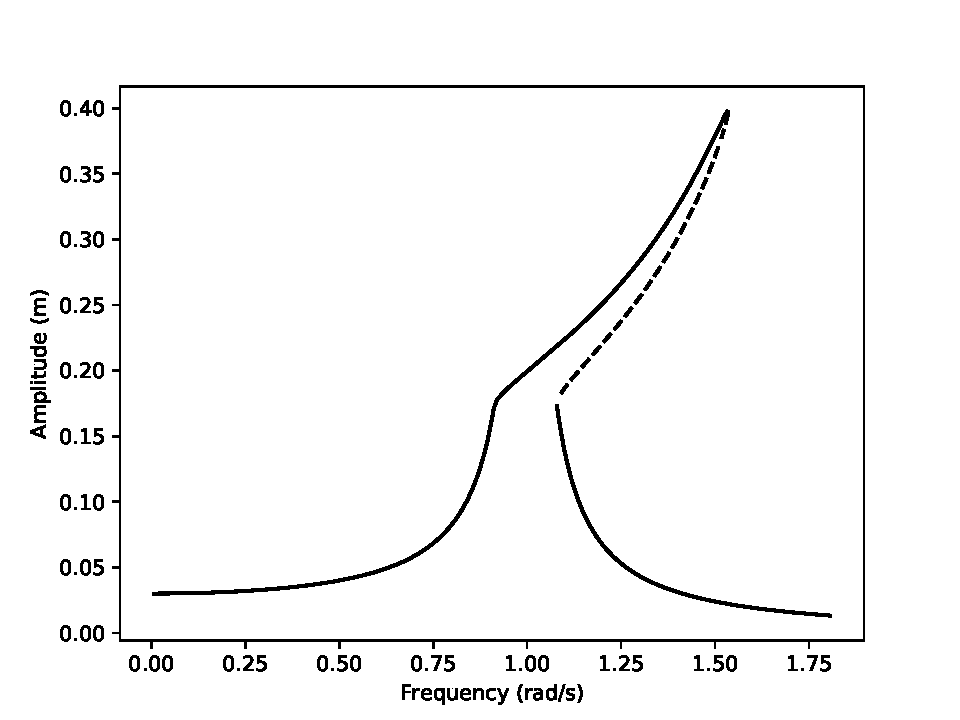
\includegraphics[width=0.7\linewidth, height=8cm]{2dof_duffing/hb_frf.tikz}
  \caption{NRFC of the coupled duffing system for $x_1$ with $f=2$N. Unstable
    branches are indicated by $- - -$. $N_H = 5, N = 512$}
  \label{fig:hb_frf_2dof}
 \end{figure}

\subsection{Summary}
\label{sec:cont_summary}

Figure \ref{fig:cont_algo} show the continuation procedure, regardless of the
the correction method. There is not much difference if implementation
complexity, but the Moore-penrose corrections saves on computional complexity.
The Pseudo-arclength method can be seen as a Moore-Penrose method for which the
correction direction is not updated.

\begin{figure}[!ht]
  \centering
  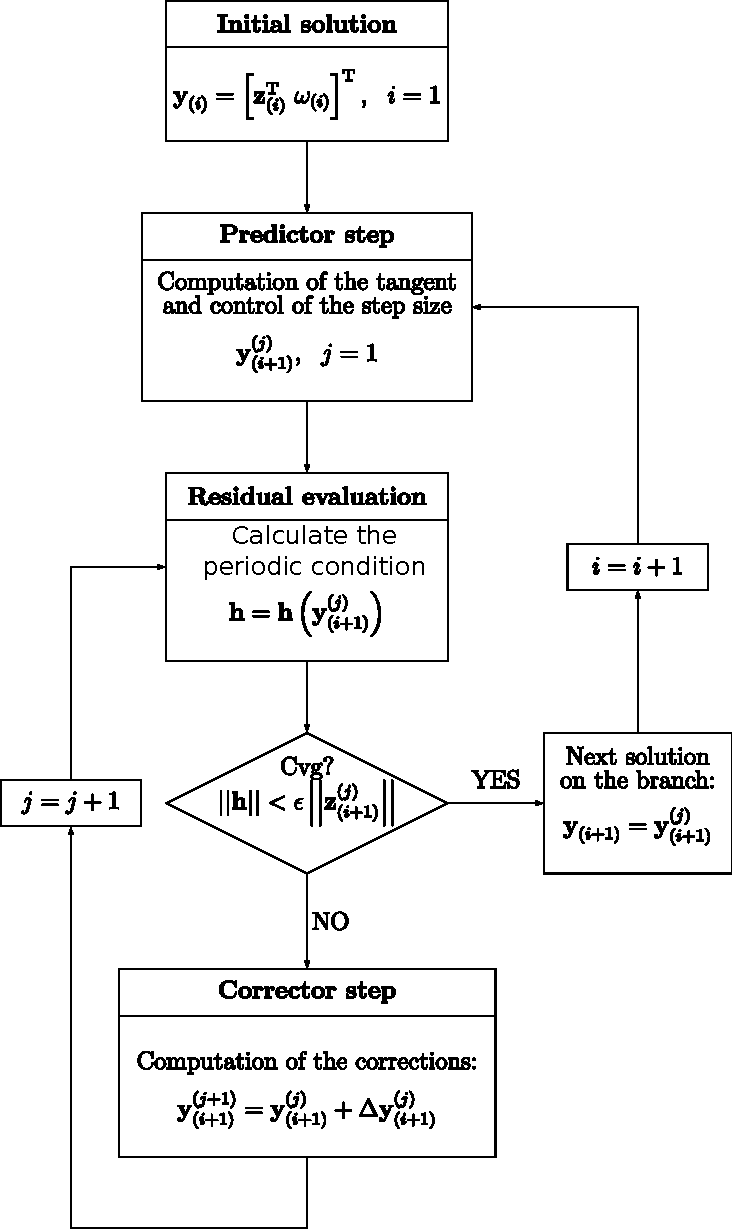
\includegraphics[width=0.7\textwidth]{continuation/continuation_diagram}
  \caption{Algorithm for Predictor-Corrector continuation of a periodic
    solution. For Moore-penrose the successive tangents are simply calculated as
  a normalization.}
  \label{fig:cont_algo}
\end{figure}



%%% Local Variables:
%%% mode: latex
%%% TeX-master: "../../report"
%%% End:
